\documentclass{article}
\usepackage{graphicx} % Required for inserting images
\usepackage[Spanish]{babel}
\usepackage{float}

\title{\textbf{\textit{Tu Primera Siembra de bacterias}}}
\author{Santiago Azael Núñez Calleja}
\date{September 25 2026}

\begin{document}

\maketitle

\section{Introducción}
\noindent Los microorganismos en la naturaleza se encuentran formando poblaciones mixtas, compuestas por diferentes tipos de bacterias, hongos o levaduras. Para estudiar de manera precisa las características de un microorganismo específico, es necesario aislarlo y obtener un cultivo puro (axénico). El cultivo puro permite identificar, analizar y caracterizar a una sola especie sin interferencia de otras presentes en la muestra original (suelo, agua, alimentos, superficies, muestras clínicas, etc.).
El proceso fundamental para lograr este aislamiento es la siembra por estría en placa, una técnica microbiológica que consiste en distribuir un inóculo sobre la superficie de un medio de cultivo sólido mediante un asa estéril, disminuyendo progresivamente la concentración de células. Tras la incubación, cada célula viable da origen a una colonia, permitiendo así observar colonias aisladas y diferenciarlas según sus características morfológicas: forma, borde, tamaño, color, consistencia, brillo y elevación. Estas colonias individuales son la base para obtener un 
\section{Principios de la siembra e inoculación}
\noindent Sembrar o inocular consiste en introducir controladamente una muestra en un medio de cultivo adecuado para permitir el crecimiento, multiplicación y posterior análisis de los microorganismos. Toda siembra debe cumplir principios de trabajo estéril:
\begin{itemize}
    \item Trabajar con técnica aséptica.
    \item Utilizar material, medios e instrumental previamente esterilizados.
    \item Manipular lo menos posible el material biológico
    \item Evitar corrientes de aire; idealmente trabajar cerca de un mechero o lámpara para crear una zona estéril.
\end{itemize}
\section{Técnica de siembra por estría (aislamiento)}
\begin{itemize}
    \item Preparación del material: Se utiliza una placa con medio de cultivo sólido (generalmente agar nutritivo u otro específico) y un asa de siembra estéril.
    \item Inoculación inicial: Se toma una pequeña cantidad del inóculo (colonia, muestra líquida o mezcla microbiana)
    \item Primer estriado: Se realizan líneas o trazos en el primer sector de la placa para distribuir el inóculo.
    \item Esterilización del asa: El asa se flamea o esteriliza para evitar arrastrar demasiadas células.
    \item Estriados sucesivos: Se arrastra material desde el área previa hacia nuevas zonas de la placa, diluyendo progresivamente las células hasta lograr colonias aisladas.
\end{itemize}
\section{Formas comunes de las bacterias}
\begin{itemize}
    \item Cocos: células esféricas 
    \item Bacilos: células alargadas en forma de bastón.
    \item Cocobacilos: intermedios entre coco y bacilo
    \item Vibriones: forma de coma o curvada.
    \item Espirilos: forma espiral rígida
    \item Espiroquetas: forma espiral flexible
\end{itemize}
\textbf{OBJETIVO}
\\ Sembrar por el método de estría cruzada, la muestra elegida 
\\
\\ \textbf{MATERIALES}
\begin{itemize}
    \item Medio de cultivo en cajas de Petri 
    \item  Asa bacteriológica
    \item Hisopos estériles
    \item Un plumón de tinta indeleble
    \item Muestras problema 
    \item Mechero Fisher
\end{itemize}
\textbf{PROCEDIMIENTO}
\begin{itemize}
    \item 1) Encender el mechero Fisher por 10 minutos
    \item 2) Utilizar isopos estériles o asa bacteriológica para realizar la siembra 
    \item 3) Rotular con un plumón indeleble de punto delgado (por ejemplo 1-SIN DESINFECTANTE, 2, 3, 4, etc diferentes DESINFECTANTES). 
    \item 4) Cerrar las cajas de Petri, apilarlas y envolver con papel estraza.
    \item 5) Poner en la incubadora de 24 a 48 horas a 37 grados. 
    \item 6) Observar resultados.
    \item 7) Toma fotografías.
    \item 8) Completa la tabla. 
\end{itemize}
\begin{figure}[H]
    \centering
    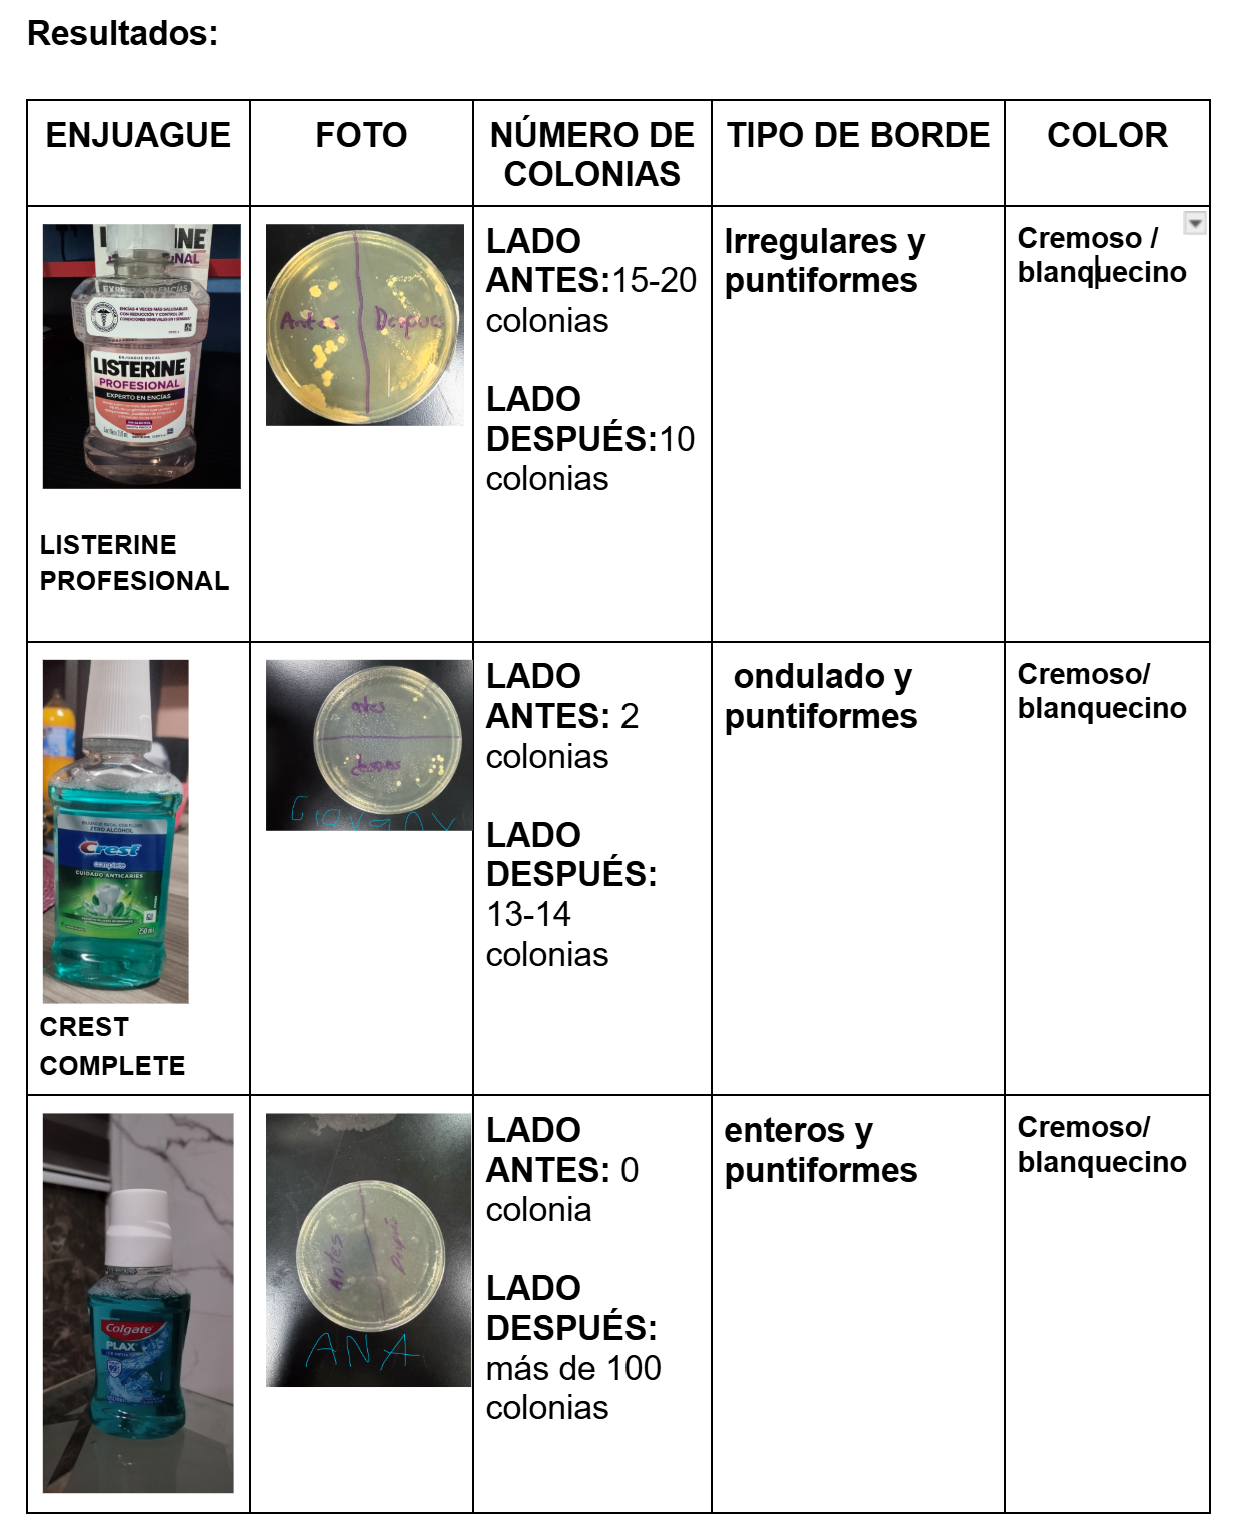
\includegraphics[width=0.85\linewidth]{Tabla parte 1.png}
    \caption{\textit{Tabla 1 Resultados}}
    \label{fig:placeholder}
\end{figure}
\begin{figure}[H]
    \centering
    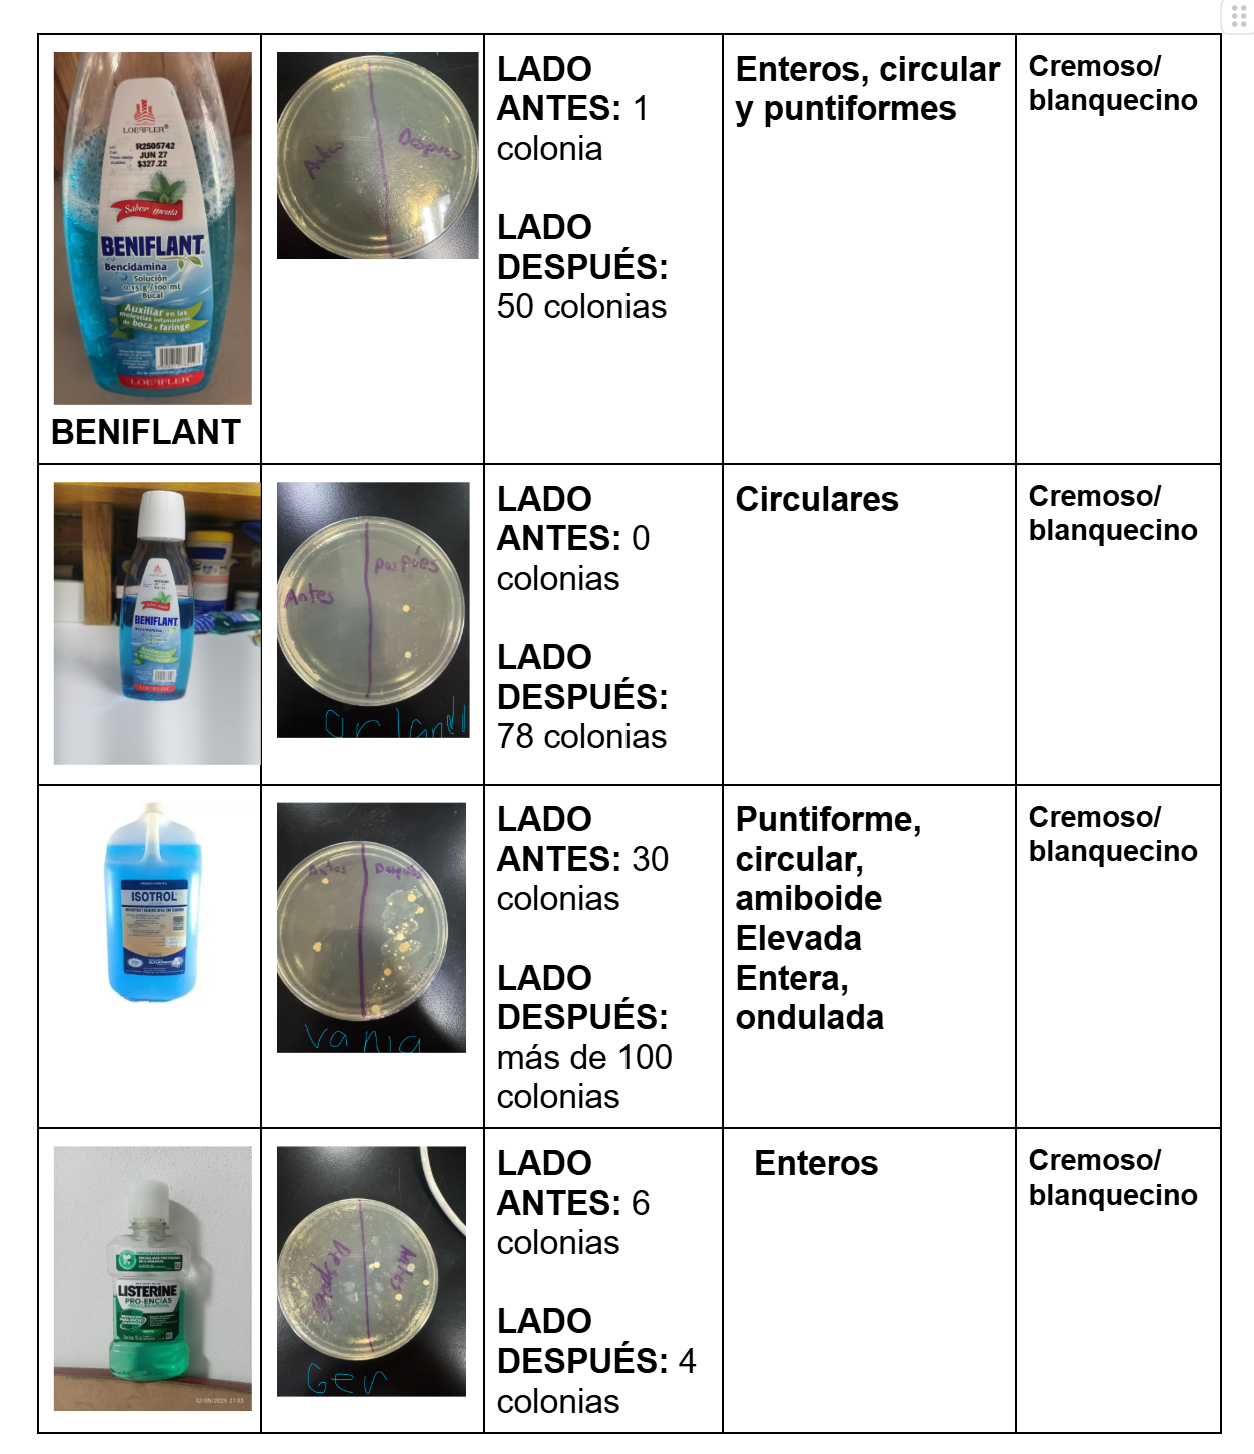
\includegraphics[width=0.85\linewidth]{Tabala parte 2.png}
    \caption{\textit{Tabla 2 Resultados}}
    \label{fig:placeholder}
\end{figure}
\section{CONCLUSIÓN}
\noindent Se logró cumplir con el objetivo de realizar la siembra mediante el método de estría cruzada, diluyendo progresivamente el inóculo sobre la superficie del medio de cultivo sólido (cajas de Petri) utilizando enjuague bucal como muestra problema. Esta técnica permitió aislar y observar las características de los microorganismos presentes, identificando colonias individuales después del proceso de incubación. La utilización de materiales como el medio de cultivo, cajas de Petri, hisopos estériles y un mechero Fisher fue indispensable para desarrollar el procedimiento en un área esterilizada y bajo condiciones controladas con el uso de una incubadora, lo que permitió obtener resultados confiables.
En cuanto al efecto del enjuague bucal, se observó que solo algunos de ellos mostraron una reducción en el crecimiento bacteriano en comparación con las muestras tomadas antes del cepillado y del enjuague. En otros casos, incluso se registró un aumento en la cantidad de bacterias después del cepillado y enjuague, lo que indica que su eficacia puede variar dependiendo del tipo de enjuague y de las condiciones de la muestra.
La metodología empleada, junto con el manejo adecuado de los medios de cultivo, permitió analizar con precisión las propiedades microbiológicas de la muestra seleccionada, cumpliendo con los objetivos planteados.
\end{document}
